% \documentclass[12pt]{article}
\documentclass[11pt]{article}
\usepackage[utf8]{inputenc}
% \usepackage[spanish]{babel}
\usepackage{amsmath}
\usepackage{enumitem}
\usepackage{xcolor}
\usepackage{cancel}
\usepackage{graphicx}
\usepackage[top=1in, bottom=1.in, left=1.in, right=1.in]{geometry}

% \usepackage{unicode-math}
% \setmathfont{XITS Math}
% 
\pagestyle{empty}
\setlength\parindent{0pt}

\begin{document}

%\vspace{1.5cm}
% \hfill{Buenos Aires, \today} \\

\begin{center}
\Large\bf
Modificación a funciones $Y^k(a,b,r)$ 
\end{center}

\section{La integral de intercambio}
La integral del término de intercambio está dada por
\begin{align}
K_{ab} &= \iint_0^{\infty}{ \phi_a(r_1)\phi_b(r_2)\frac{1}{\left|\mathbf{r}_1-\mathbf{r}_2\right|}\phi_a(r_2)\phi_b(r_1)}\,d\mathbf{r}_1\,d\mathbf{r}_2\\
 &= \int_0^{\infty} P_a(r_1)P_b(r_1) \left[ \int_0^{\infty} \frac{P_b(r_2)P_b(r_2)}{\left|\mathbf{r}_1-\mathbf{r}_2\right|}\,dr_2 \right] \,dr_1 \times \int \mathcal{Y}(a,b,\Omega_1,\Omega_2)\,d\Omega_1\,d\Omega_2\,,
\end{align}
donde $\mathcal{Y}(a,b,\Omega_1,\Omega_2)$ es una función que depende de las partes angulares correspondientes a $\phi_a$ y $\phi_b$. 
Usando el desarrollo multipolar,
\begin{align}
 \frac{1}{\left|\mathbf{r}-\mathbf{r}'\right|} &= \sum_{k=0}^{\infty}\sum_{m'=-k}^{k}{\frac{{r_<}^k}{r_>^{k+1}} 
\frac{4\pi}{2k+1}{Y_k^{m'}}^* (\theta,\phi){Y_k^{m'}}(\theta',\phi') } \\
 &=\sum_{k=0}^{\infty}{\frac{{r_<}^k}{{r_>}^{k+1}}P_l(\cos\theta)} \,.
\end{align}
Entonces, la parte radial de la integral de intercambio resulta
\begin{align}
K_{ab}' &= \int_0^{\infty} P_a(r_1)P_b(r_1) \left[ \int_0^{\infty} \frac{{r_<}^k}{{r_>}^{k+1}}P_b(r_2)P_b(r_2)\,dr_2 \right] dr_1\,.
\label{eq:Kab_radial}
\end{align}


\subsection{Las funciones $Y_{ab}^k(r)$}

Por definición,
\begin{align}
 \frac{Y_{ab}^k(r) }{r}
 &= \int_0^{\infty} \frac{r_<^k}{r_>^{k+1}}P_a(t)P_b(t)\,dt \\
 &= \int_0^r \frac{t^k}{r^{k+1}} P_a(t)P_b(t)\,dt 
  + \int_r^{\infty} \frac{r^k}{t^{k+1}} P_a(t)P_b(t)\,dt \\
 &=\frac{1}{r} \left[ \int_0^r \left(\frac{t}{r}\right)^k P_a(t)P_b(t)\,dt
  + \int_r^{\infty} \left(\frac{r}{t}\right)^{k+1} P_a(t)P_b(t)\,dt \right]\\
 \Rightarrow\quad Y_{ab}^k(r) &= \frac{1}{r^k} \int_0^r t^k P_a(t)P_b(t)\,dt
  + r^{k+1} \int_r^{\infty} \frac{P_a(t)P_b(t)}{t^{k+1}}\,dt \,.
\end{align}
Definiendo la función $Z_{ab}^k(r)$ tal que
\begin{align}
 Z_{ab}^k(r) &= \frac{1}{r^k} \int_0^r t^k P_a(t)P_b(t)\,dt\,,
\label{eq:Zabk}
\end{align}
es posible expresar $Y_{ab}^k(r)$ en términos de $Z_{ab}^k(r)$
\begin{align}
 Y_{ab}^k(r) &= Z_{ab}^k(r) 
 + r^{k+1} \int_r^{\infty} \frac{P_a(t)P_b(t)}{t^{k+1}}\,dt \,.
\label{eq:Yabk}
\end{align}

\subsection{Ecuaciones diferenciales de $Y_{ab}^k(r)$}

La primera derivada de la función $Z_{ab}^k(r)$ resulta
\begin{align}
 \frac{d\,Z_{ab}^k(r)}{dr} 
 &= \frac{d}{dr} \left[ \frac{1}{r^k} \int_0^r t^k P_a(t)P_b(t)\,dt \right] \\
 &= -\frac{k}{r^{k+1}}\int_0^r t^k P_a(t)P_b(t)\,dt + \frac{1}{r^k} \left[ r^k P_a(r)P_b(r) \right] \\
 &= P_a(r)P_b(r) -\frac{k}{r^{k+1}}\int_0^r t^k P_a(t)P_b(t)\,dt \\
 \Rightarrow\quad \frac{d\,Z_{ab}^k(r)}{dr} &= P_a(r)P_b(r) - \frac{k}{r} Z_{ab}^k(r)  \,.
 \label{eq:dZkab_A}
\end{align}
En donde se usa el hecho que
\begin{align}
 \frac{d}{dr} \int_0^r f(t)\,dt = f(r)\,.
\end{align}

Por otro lado, la primera derivada de la la función $Y_{ab}^k(r)$ está dada por
\begin{align}
 \frac{d\,Y_{ab}^k }{dr}
 &= \frac{d}{dr} \left[ Z_{ab}^k(r) 
 + r^{k+1} \int_r^{\infty} \frac{P_a(t)P_b(t)}{t^{k+1}}\,dt \right] \\
 &= \frac{d\, Z_{ab}^k(r)}{dr} + (k+1) r^k \int_r^{\infty} \frac{P_a(t)P_b(t)}{t^{k+1}}\,dt 
 - r^{k+1}\left[ \frac{1}{r^{k+1}} P_a(r)P_b(r) \right] \\
 &= \left[ P_a(r)P_b(r) - \frac{k}{r} Z_{ab}^k(r) \right]
 + (k+1) r^k \int_r^{\infty} \frac{P_a(t)P_b(t)}{t^{k+1}}\,dt - P_a(r)P_b(r) \\
 &= -\frac{k}{r} Z_{ab}^k(r) 
 + (k+1) r^k \int_r^{\infty} \frac{P_a(t)P_b(t)}{t^{k+1}}\,dt \\
 &= -\frac{k}{r} Z_{ab}^k(r)  \left[ - \frac{k+1}{r} Z_{ab}^k(r) + \frac{k+1}{r} Z_{ab}^k(r) \right]
 + (k+1) r^k \int_r^{\infty} \frac{P_a(t)P_b(t)}{t^{k+1}}\,dt  \\
 &= -\frac{2k+1}{r} Z_{ab}^k(r) + \frac{k+1}{r} Z_{ab}^k(r)
 + \frac{k+1}{r} r^{k+1} \int_r^{\infty} \frac{P_a(t)P_b(t)}{t^{k+1}}\,dt \\
 &= -\frac{2k+1}{r} Z_{ab}^k(r) + \frac{k+1}{r} \left[ Z_{ab}^k(r)
 + r^{k+1} \int_r^{\infty} \frac{P_a(t)P_b(t)}{t^{k+1}}\,dt \right] \\
 \Rightarrow\quad\frac{d\,Y_{ab}^k }{dr}&= -\frac{2k+1}{r} Z_{ab}^k(r) + \frac{k+1}{r} Y_{ab}^k(r)\,.
 \label{eq:dYkab_A}
\end{align}

\subsection{Cambio de variable}
Haciendo un cambio de variables, tal que
\begin{equation}
r=e^{\rho}\,,
\label{eq:r-rho}
\end{equation}
entonces,
\begin{equation}
 \frac{dr}{d\rho}=r\,.
\end{equation}
Aplicando la regla de la cadena,  
\begin{align}
 \frac{df^k}{dr}=\frac{df^k}{d\rho}\frac{d\rho}{dr} \\
 \quad\Rightarrow\quad 
 \frac{df^k}{d\rho}&=\frac{df^k}{dr}\frac{dr}{d\rho}\\
 &=r\frac{df^k}{dr}\,.
\end{align}

Entonces, siendo $P_i(r)=\sqrt{r}\,\overline{P}_i(\rho)$, la Ec. (\ref{eq:dZkab_A}) resulta
\begin{align}
 \frac{d\,Z_{ab}^k}{d\rho}  &=  r^2\,\overline{P}_a(\rho)\overline{P}_b(\rho) - k Z_{ab}^k(\rho)\,.
 \label{eq:Zabk_B}
\end{align}
Mientras que la Ec.~(\ref{eq:dYkab_A}) se reescribe como
\begin{align}
 \frac{d\,Y_{ab}^k }{d\rho} &=  -[2k+1] Z_{ab}^k(\rho) + [k+1] Y_{ab}^k(\rho)\,.
 \label{eq:Yabk_B}
\end{align}

\subsection{Factor de integración}

Fischer, página 232.

\section{Modificación a la integral de intercambio}

Modificando la integral de intercambio de manera tal que introducimos una función exponencial decreciente dependiente del parámetro $\alpha$,
\begin{align}
K_{ab} &= \iint_0^{\infty}{ \phi_a(r_1)\phi_b(r_2)\frac{e^{-\alpha(r_1-r_2)}}{\left|\mathbf{r}_1-\mathbf{r}_2\right|}\phi_a(r_2)\phi_b(r_1)}\,d\mathbf{r}_1\,d\mathbf{r}_2\,.
\end{align}
La parte radial correspondiente a $K_{ab}$ resulta
\begin{align}
 K_{ab}' &= \int_0^{\infty} e^{-\alpha r_1} P_a(r_1)P_b(r_1) \left[ \int_0^{\infty} e^{\alpha r_2}\,\frac{{r_<}^k}{{r_>}^{k+1}} P_b(r_2)P_b(r_2)\,dr_2 \right] dr_1\,.
\end{align}

\subsection{Modificación a las funciones $Y_{ab}^k(r)$}

{\color{red}\bf Me falta esta derivación...}

\subsection{Ecuaciones diferenciales de $Y_{ab}^k(r)$}

{\color{red}\bf Me falta esta derivación...}

\vspace{0.25cm}
Así, la ecuación resultante para $Z_{ab}^k(r)$ es
\begin{align}
 \frac{d\,Z_{ab}^k}{dr}=P_a(r)P_b(r)-\left[\alpha+\frac{k}{r}\right] Z_{ab}^k(r)\,.
 \label{eq:dZabk_alpha}
\end{align}
Y la ecuación diferencial modificada de $Y_{ab}^k(r)$ resulta
\begin{align}
 \frac{d\,Y_{ab}^k}{dr}=-\left[2\alpha+\frac{2k+1}{r}\right]Z_{ab}^k(r) + \left[\alpha+\frac{k+1}{r}\right] Y_{ab}^k(r)\,.
 \label{eq:dYabk_alpha}
\end{align}

\subsection{Cambio de variable}

Haciendo el mismo cambio de variable dado por la 
Ec.~(\ref{eq:r-rho}), entonces la Ec.~(\ref{eq:dZabk_alpha})
resulta
\begin{align}
 \frac{d\,Z_{ab}^k}{d\rho}=r\,\overline{P}_a\overline{P}_b - \left(r\alpha+k\right) Z_{ab}^k(\rho)\,.
 \label{eq:dZabk_rho_alpha}
\end{align}
y la Ec.~(\ref{eq:dYabk_alpha}) se reescribe como
\begin{align}
 \color{red} 
 \frac{d\,Y_{ab}^k}{d\rho}=-\left[2\alpha r+2k+1\right]Z_{ab}^k(\rho)+\left[\alpha r+k+1\right]Y_{ab}^k(\rho)
 \label{eq:dYabk_rho_alpha}
\end{align}

\subsection{Factor de integración}
Siendo 
\begin{equation}
 f_1=e^{\alpha r+k\rho}\,,
\end{equation}
el factor de integración de $Z_{ab}^k$, entonces
\begin{align}
 \frac{d\left(f_1\,Z_{ab}^k\right)}{d\rho} 
 &=\frac{df_1}{d\rho} Z_{ab}^k + f_1 \frac{d\, Z_{ab}^k}{d\rho}
\end{align}
Reemplazando la Ec. (\ref{eq:dZabk_rho_alpha}),
\begin{align}
 \frac{d\left(f_1\,Z_{ab}^k\right)}{d\rho} 
 &=\frac{df_1}{d\rho} Z_{ab}^k(\rho) + f_1 \left[r\,\overline{P}_a\overline{P}_b - \left(r\alpha+k\right) Z_{ab}^k(\rho)\right]\\
 &=\frac{df_1}{d\rho} Z_{ab}^k(\rho) + r\,\overline{P}_a\overline{P}_b\,f_1 - \left(r\alpha+k\right)f_1\, Z_{ab}^k(\rho)\\
 &=\cancel{(\alpha r+k)e^{\alpha r+k\rho} Z_{ab}^k(\rho)} + r\,\overline{P}_a\overline{P}_b\,e^{\alpha r+k\rho} - \cancel{\left(r\alpha+k\right)e^{\alpha r+k\rho}\, Z_{ab}^k(\rho)} \\
 \Rightarrow\quad \frac{d\left(f_1\,Z_{ab}^k\right)}{d\rho} 
 &= r\,\overline{P}_a\overline{P}_b f_1 
 \label{eq:df1Zk_rho}
\end{align}
Entonces, 
\begin{align}
 \frac{df_1}{d\rho} Z_{ab}^k &= \left(r\alpha+k\right)f_1\, Z_{ab}^k(\rho) \\
 \frac{1}{f_1}\frac{df_1}{d\rho}&=r\alpha+k \\
 d \ln f_1 &=(\alpha\,e^{\rho} +k)\,d\rho \\
 \ln f_1 &=\int (\alpha\,e^{\rho}+k)\,d\rho \\
 \ln f_1 &=\alpha\,e^{\rho}+k\rho \\
 \Rightarrow\quad f_1(\rho)&=e^{\alpha r+k\rho}
\end{align}
Así, $f_1$ es efectivamente un factor de integración. Luego, de (\ref{eq:df1Zk_rho})
\begin{align}
 \frac{d\left[e^{\alpha r+k\rho}\,Z_{ab}^k\right]}{d\rho} &= r\,\overline{P}_a\overline{P}_b e^{\alpha r+k\rho} 
\end{align}
Integrando,
\begin{align}
 \int_{\rho_j}^{\rho_{j+m}} d\left[e^{\alpha r+k\rho}\,Z_{ab}^k\right] &= \int_{\rho_j}^{\rho_{j+m}} r\,\overline{P}_a\overline{P}_b\,e^{\alpha r+k\rho}\,d\rho \\
 e^{\alpha r_{j+m}+k\rho_{j+m}}\,Z_{ab}^k(\rho_{j+m}) - e^{\alpha r_j+k\rho_j}\,Z_{ab}^k(\rho_j)&= \int_{\rho_j}^{\rho_{j+m}} r\,\overline{P}_a\overline{P}_b\,e^{\alpha r+k\rho}\,d\rho 
\end{align}
Despejando $Z_{ab}^k(\rho_{j+m})$,
\begin{align} 
 Z_{ab}^k(\rho_{j+m}) 
 &= e^{-\left[\alpha r_{j+m}+k\rho_{j+m}\right]} \left[e^{\alpha r_j+k\rho_j}\,Z_{ab}^k(\rho_j) + \int_{\rho_j}^{\rho_{j+m}} r\,\overline{P}_a\overline{P}_b\, e^{\alpha r+k\rho}\,d\rho \right] \\ 
 &= e^{-\alpha r_{j+m}}\left[e^{\alpha r_j+k\rho_j}e^{-k\rho_{j+m}} \,Z_{ab}^k(\rho_j) + \int_{\rho_j}^{\rho_{j+m}} r\,\overline{P}_a\overline{P}_b\, e^{\alpha r+k\rho}e^{-k\rho_{j+m}} \,d\rho \right] \\ 
 &= e^{-\alpha r_{j+m}}\left[e^{\alpha r_j}e^{-k(\rho_{j+m}-\rho_j)} \,Z_{ab}^k(\rho_j) + \int_{\rho_j}^{\rho_{j+m}} r\,\overline{P}_a\overline{P}_b\, e^{\alpha r}e^{k(\rho-\rho_{j+m})} \,d\rho \right] 
\end{align}
Siendo $mh=\rho_{j+m}-\rho_j$,
\begin{align}
 Z_{ab}^k(\rho_{j+m}) 
 &= {\color{red} e^{-\alpha r_{j+m}} }\left[ {\color{red} e^{\alpha r_j} } e^{-kmh}\,Z_{ab}^k(\rho_j) + \int_{\rho_j}^{\rho_{j+m}} r\,\overline{P}_a\overline{P}_b\,{\color{red} e^{\alpha r}}e^{k(\rho-\rho_{j+m})}\,d\rho \right] \,,
\end{align}
donde los términos en rojo son los nuevos términos que aparecen 
al incluir la modificación en la integral de intercambio.

\vspace{0.25cm}
Siendo 
\begin{equation}
 f_2=e^{-[\alpha r + (k+1)\rho]}
\end{equation}
el factor de integración de $Y_{ab}^k$, tengo que
\begin{align}
 \frac{d\,(f_2\,Y_{ab}^k)}{d\rho}
 &=\frac{df_2}{d\rho}\, Y_{ab}^k(\rho) + f_2 \,\frac{d\,Y_{ab}^k}{d\rho} 
\end{align}
Reemplazando la Ec. (\ref{eq:dYabk_rho_alpha}),
\begin{align}
 \frac{d\,(f_2\,Y_{ab}^k)}{d\rho}
 &=\frac{df_2}{d\rho}\, Y_{ab}^k
 + f_2 \left[-\left(2r\alpha+2k+1\right)Z_{ab}^k+\left(r\alpha+k+1\right)Y_{ab}^k \right] \\
 &=\cancel{-\left(\alpha r +k+1\right)f_2\, Y_{ab}^k}
 - \left(2r\alpha+2k+1\right)f_2 \,Z_{ab}^k
 +\cancel{\left(r\alpha+k+1\right)f_2\,Y_{ab}^k} \\
 &=-\left(2r\alpha+2k+1\right) e^{-[\alpha r + (k+1)\rho]} \,Z_{ab}^k
\end{align}
Nuevamente, integrando entre $\rho_j$ y $\rho_{j+m}$,
\begin{align}
 \int_{\rho_j}^{\rho_{j+m}} 
 d\,(e^{-[\alpha r + (k+1)\rho]}\,Y_{ab}^k)
 = -\int_{\rho_j}^{\rho_{j+m}}& \left(2r\alpha+2k+1\right) e^{-[\alpha r + (k+1)\rho]} \,Z_{ab}^k\, d\rho \\
 e^{-[\alpha r_{j+m} + (k+1)\rho_{j+m}]}\,Y_{ab}^k(\rho_{j+m})-e^{-[\alpha r_j + (k+1)\rho_j]}\,Y_{ab}^k(\rho_j) \nonumber
 &= \\ -\int_{\rho_j}^{\rho_{j+m}} & \left(2r\alpha+2k+1\right) e^{-[\alpha r + (k+1)\rho]} \,Z_{ab}^k\, d\rho 
\end{align}
Despejando $Y_{ab}^k(\rho_j)$,
\begin{align}
 Y_{ab}^k(\rho_j)
 =e^{\alpha r_j + (k+1)\rho_j}\Bigg[ e^{-[\alpha r_{j+m} + (k+1)\rho_{j+m}]}\,& Y_{ab}^k(\rho_{j+m}) \nonumber \\ 
 & +\int_{\rho_j}^{\rho_{j+m}} \left(2r\alpha+2k+1\right) e^{-[\alpha r + (k+1)\rho]} \,Z_{ab}^k\, d\rho \Bigg] \\
 =e^{\alpha r_j}\Bigg[ e^{-\alpha r_{j+m}}e^{-(k+1)\rho_{j+m}} e^{(k+1)\rho_j} & Y_{ab}^k(\rho_{j+m}) \nonumber \\ 
 + \int_{\rho_j}^{\rho_{j+m}} & \left(2r\alpha+2k+1\right) e^{-\alpha r}e^{-(k+1)\rho} e^{(k+1)\rho_j}\,Z_{ab}^k\, d\rho \Bigg] \\
 = e^{\alpha r_j}\Bigg[ e^{-\alpha r_{j+m}}e^{-(k+1)(\rho_{j+m}-\rho_j)} Y_{ab}^k&(\rho_{j+m}) \nonumber \\ 
 + \int_{\rho_j}^{\rho_{j+m}} & \left(2r\alpha+2k+1\right) e^{-\alpha r}e^{-(k+1)(\rho-\rho_j)}\,Z_{ab}^k\, d\rho \Bigg] 
\end{align}
Siendo $mh=\rho_{j+m}-\rho_j$,
\begin{align}
 Y_{ab}^k(\rho_j)&={\color{red}e^{\alpha r_j}} \left[ {\color{red} e^{-\alpha r_{j+m}}}e^{-(k+1)mh}\,Y_{ab}^k(\rho_{j+m}) + \left({\color{red}2r\alpha}+2k+1\right) \int_{\rho_j}^{\rho_{j+m}} {\color{red}e^{-\alpha r}}\,e^{-(k+1)(\rho-\rho_j)}\,Z_{ab}^k\, d\rho \right]
\end{align}
donde los términos en rojo son los nuevos términos que aparecen 
al incluir la modificación en la integral de intercambio.

\newpage
Pasos a seguir:
\begin{figure}[h]
 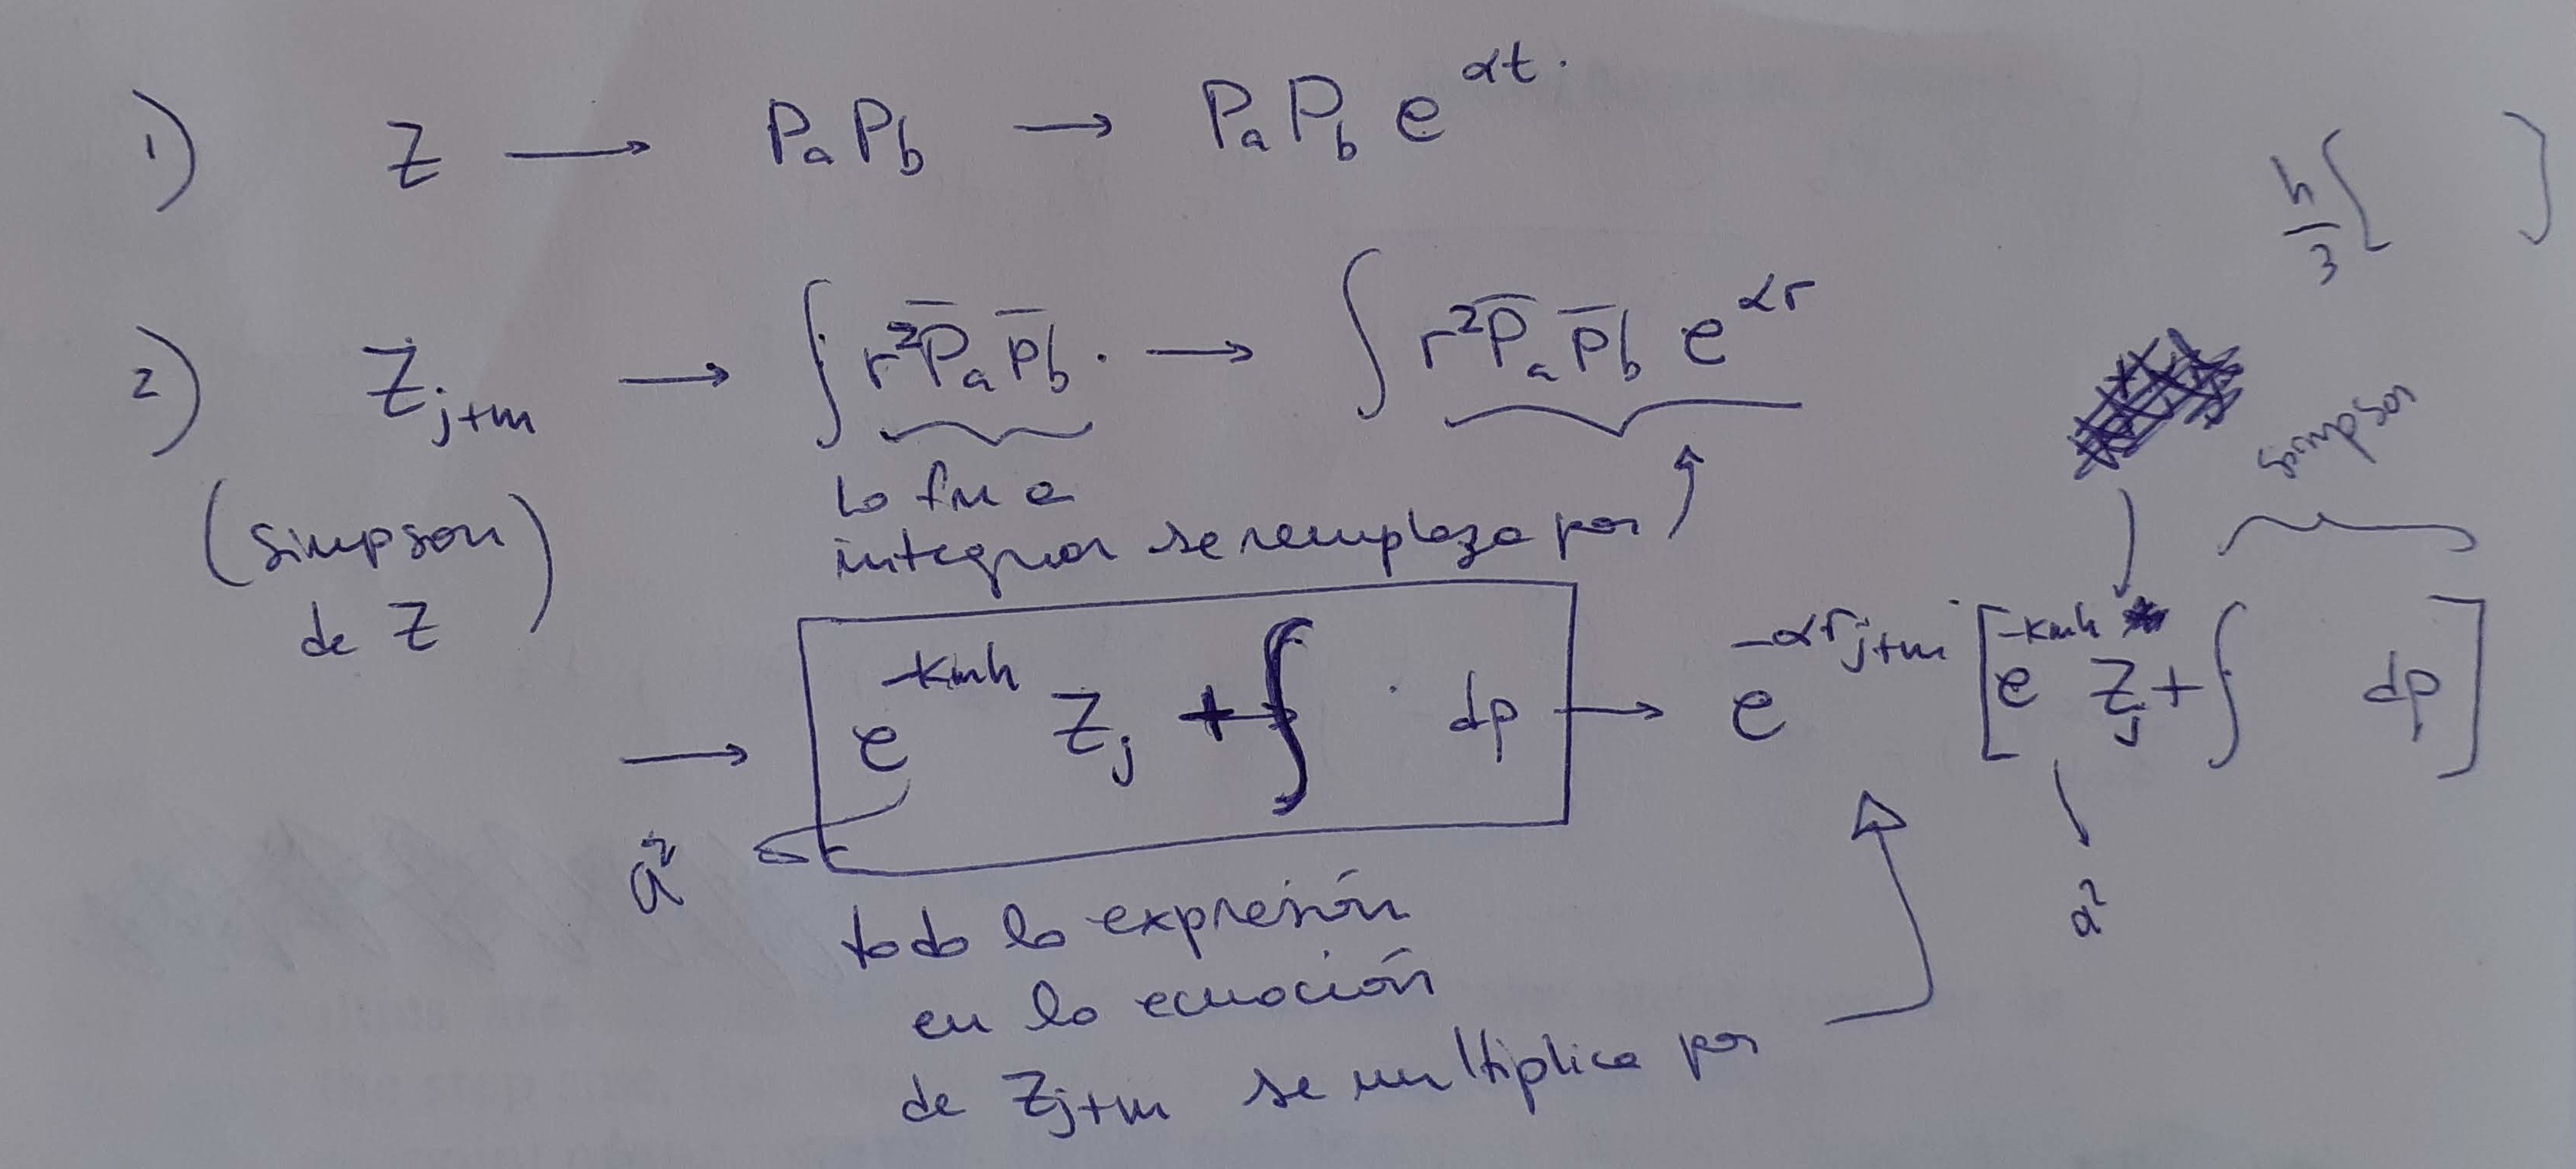
\includegraphics[width=\textwidth]{Z.jpg} \\
 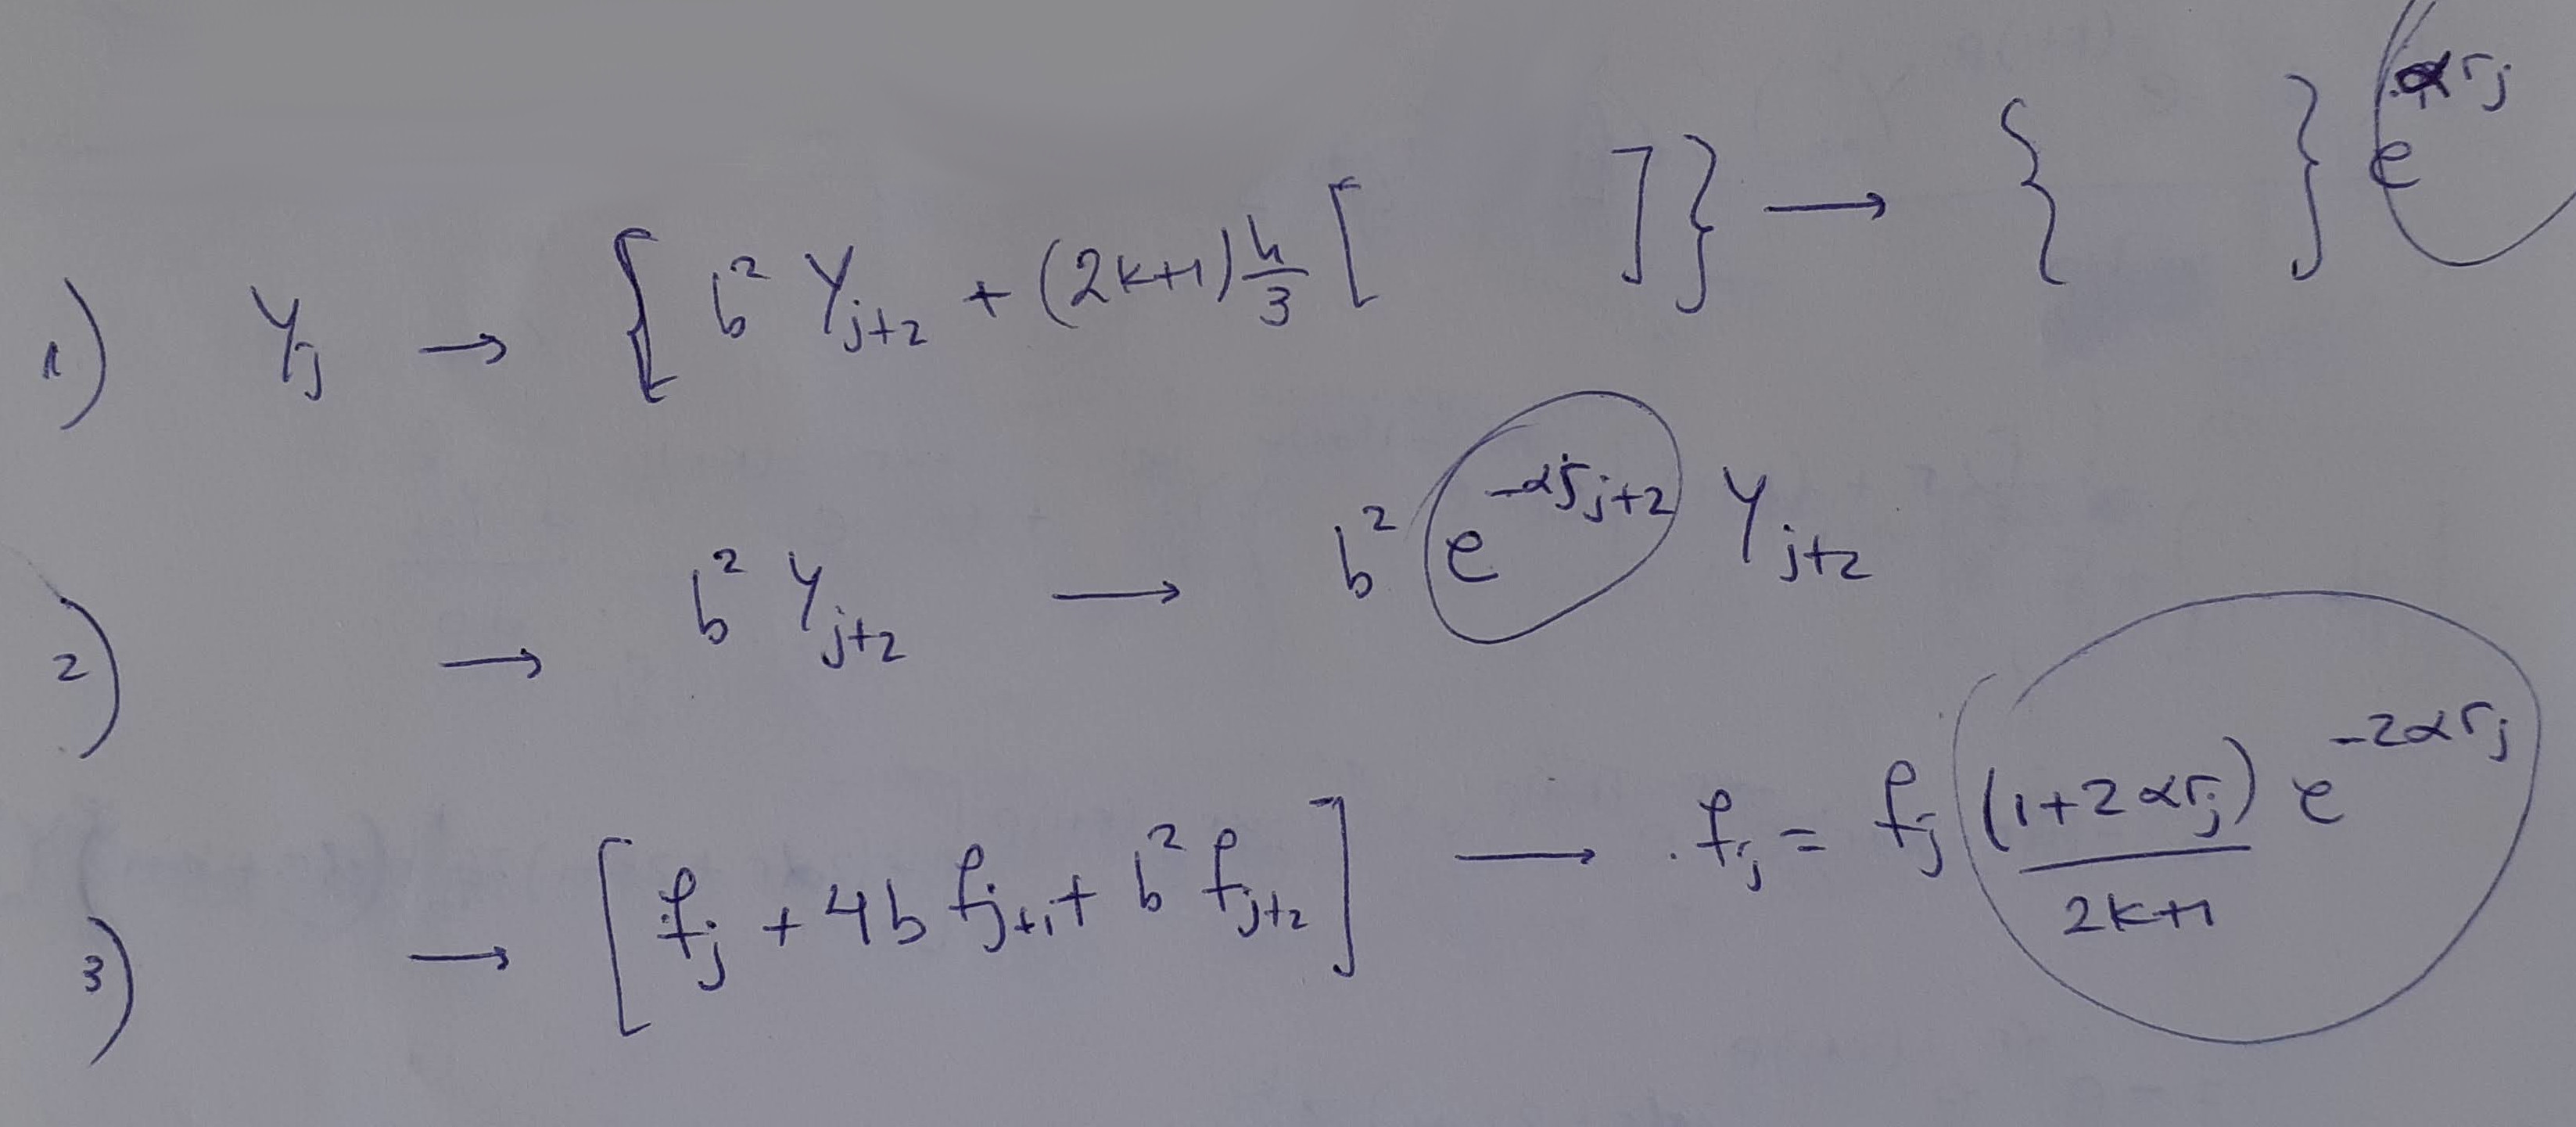
\includegraphics[width=\textwidth]{Y.jpg}
\end{figure}


\end{document}
